\section{PD szabályzó tervezése}

%{{{ Bevezetés, értelmezés

\Aref{fig:pi-hatasvazlat}. ábrában a $\fn{W}_\text{c}$ szabályzót cseréljük ki
egy PD szabályzóra, melynek átviteli függvénye
\begin{equation}
	\fn{W}_\text{c} = P\frac{T_\text{D}s+1}{nT_\text{D}s+1}.
\end{equation}
A deriváló tag időállandóját a szabályozott szakasz második legnagyobb időállandójának
célszerű megválasztani, ami $T_\text{D} = 1,3825\cdot 10^{-4}$.
Továbbá $n=\vartheta_3=40,827$ adott.

%}}}

%{{{ A zárt szabályozási kör egyenletei
\subsection{A zárt szabályozási kör egyenletei}

Jelöljük az előrevezető ág átviteli függvényét $\fn{W}_\text{x}$-val.
A zárt szabályozási kör átviteli függvénye
\begin{equation}\label{eq:W-x}
	\fn{W}_\text{o} = \frac{\fn{W}_\text{x}}{1 + \fn{W}_\text{x}} =
	\frac{P\, \ke\, \km\, \left(T_\text{D}\, s + 1\right)}{\left(\frac{P\, \ke\, \km\, \left(T_\text{D}\, s + 1\right)}{\left(T_\text{D}\, n\, s + 1\right)\, \left(\Ja\, \La\, s^2 + \Ja\, \Ra\, s + \ke\, \km\right)} + 1\right)\, \left(T_\text{D}\, n\, s + 1\right)\, \left(\Ja\, \La\, s^2 + \Ja\, \Ra\, s + \ke\, \km\right)}
\end{equation}

A zárt szabályozási kör karakterisztikus egyenlete \aref{eq:W-x}. egyenlet nevezője,
ami nullával egyenlő.
\begin{equation}
	\ke\, \km + \Ja\, \Ra\, s + P\, \ke\, \km + \Ja\, \La\, s^2 + P\, T_\text{D}\, \ke\, \km\, s + T_\text{D}\, \ke\, \km\, n\, s + \Ja\, \La\, T_\text{D}\, n\, s^3 + \Ja\, \Ra\, T_\text{D}\, n\, s^2 = 0
\end{equation}
%}}}

%{{{ Stabilitás a P függvényében
\subsection{Stabilitás a körerősítés függvényében}

Rajzoljuk ki a pólusok valós részeit a körerősítés függvényében.
\Aref{fig:poles2}. ábrán látható, hogy minden $P>0$ értékre a pólusok
negatív része valós, tehát a rendszer stabil.
\begin{figure}[H]
	\centering
	\begin{subfigure}{.49\textwidth}
		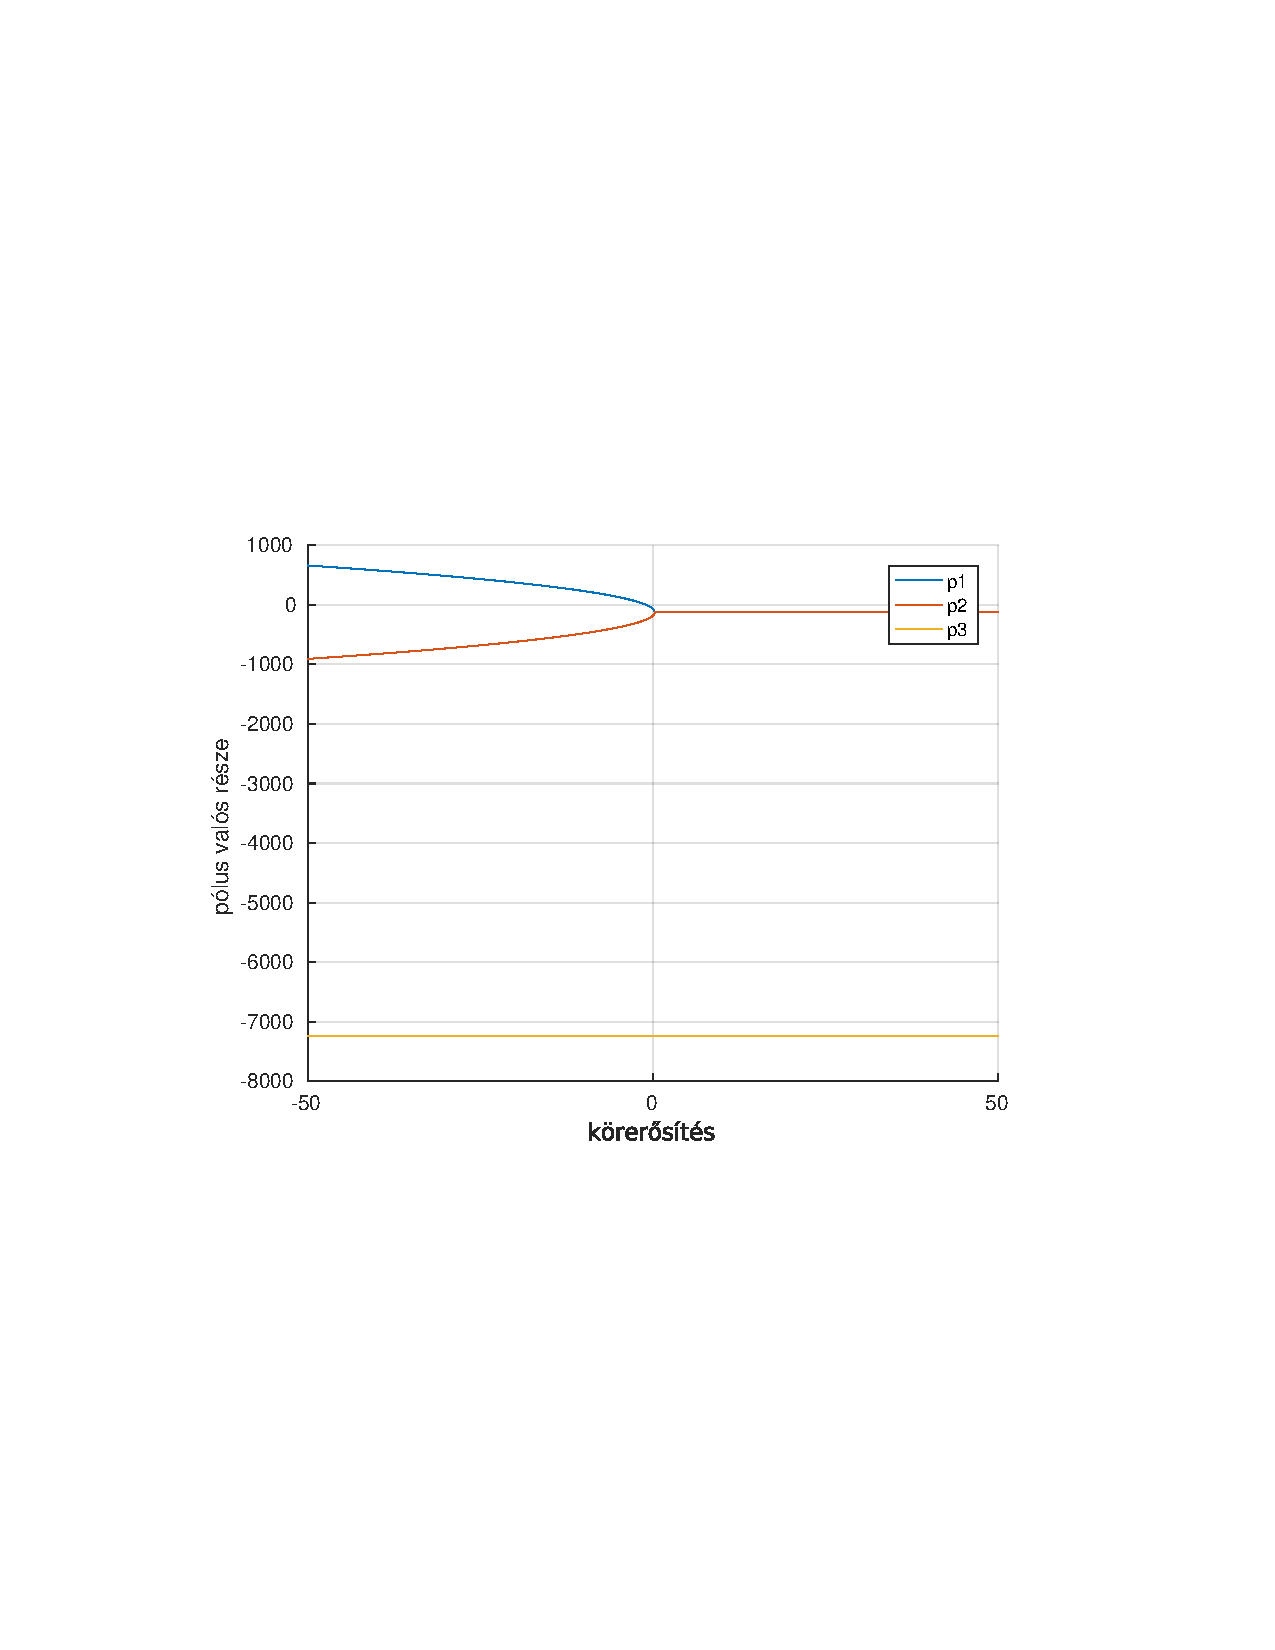
\includegraphics[width=\linewidth, trim=90 240 100 252, clip]{polus2}
		\caption{Lényeges $P$ értékek}
	\end{subfigure}
	\begin{subfigure}{.49\textwidth}
		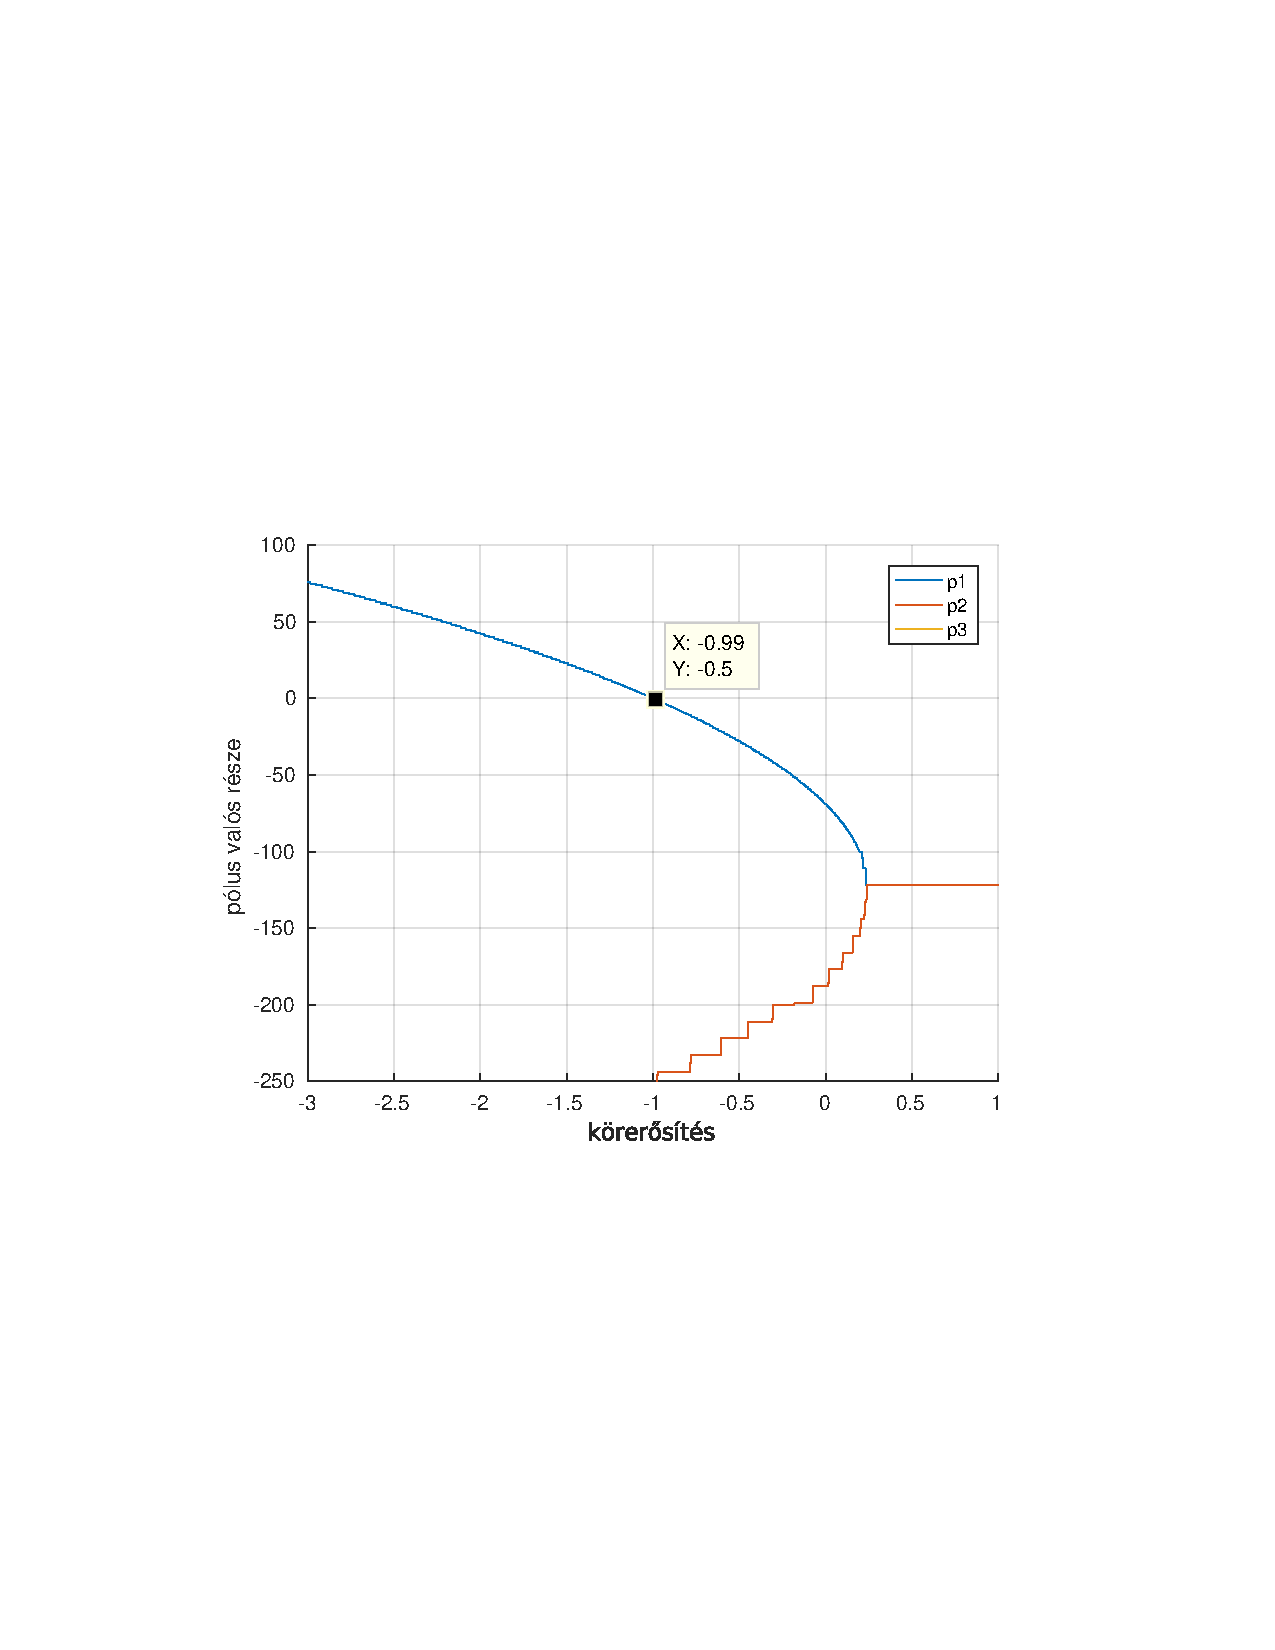
\includegraphics[width=\linewidth, trim=90 240 100 252, clip]{polus2-big}
		\caption{0 körüli $P$-k}
	\end{subfigure}
	\caption{Pólusok valós része a körerősítés függvényében}
	\label{fig:poles2}
\end{figure}

%}}}

%{{{ Megadott körerősítés esetén Bode-diagram és fázistartalék
\subsection{Megadott körerősítés esetén Bode-diagram és fázistartalék}

Válasszuk a körerősítést $P=\vartheta_4 = 40,827$-re.
Ennek a rendszernek a Bode-diagramját mutatja \aref{fig:bode2}. ábra.
A \verb|margin| függvényt használva megkapjuk a fázistartalékot,
ami $\varphi_\text{m}=90,3^\circ$.

\begin{figure}[H]
	\centering
	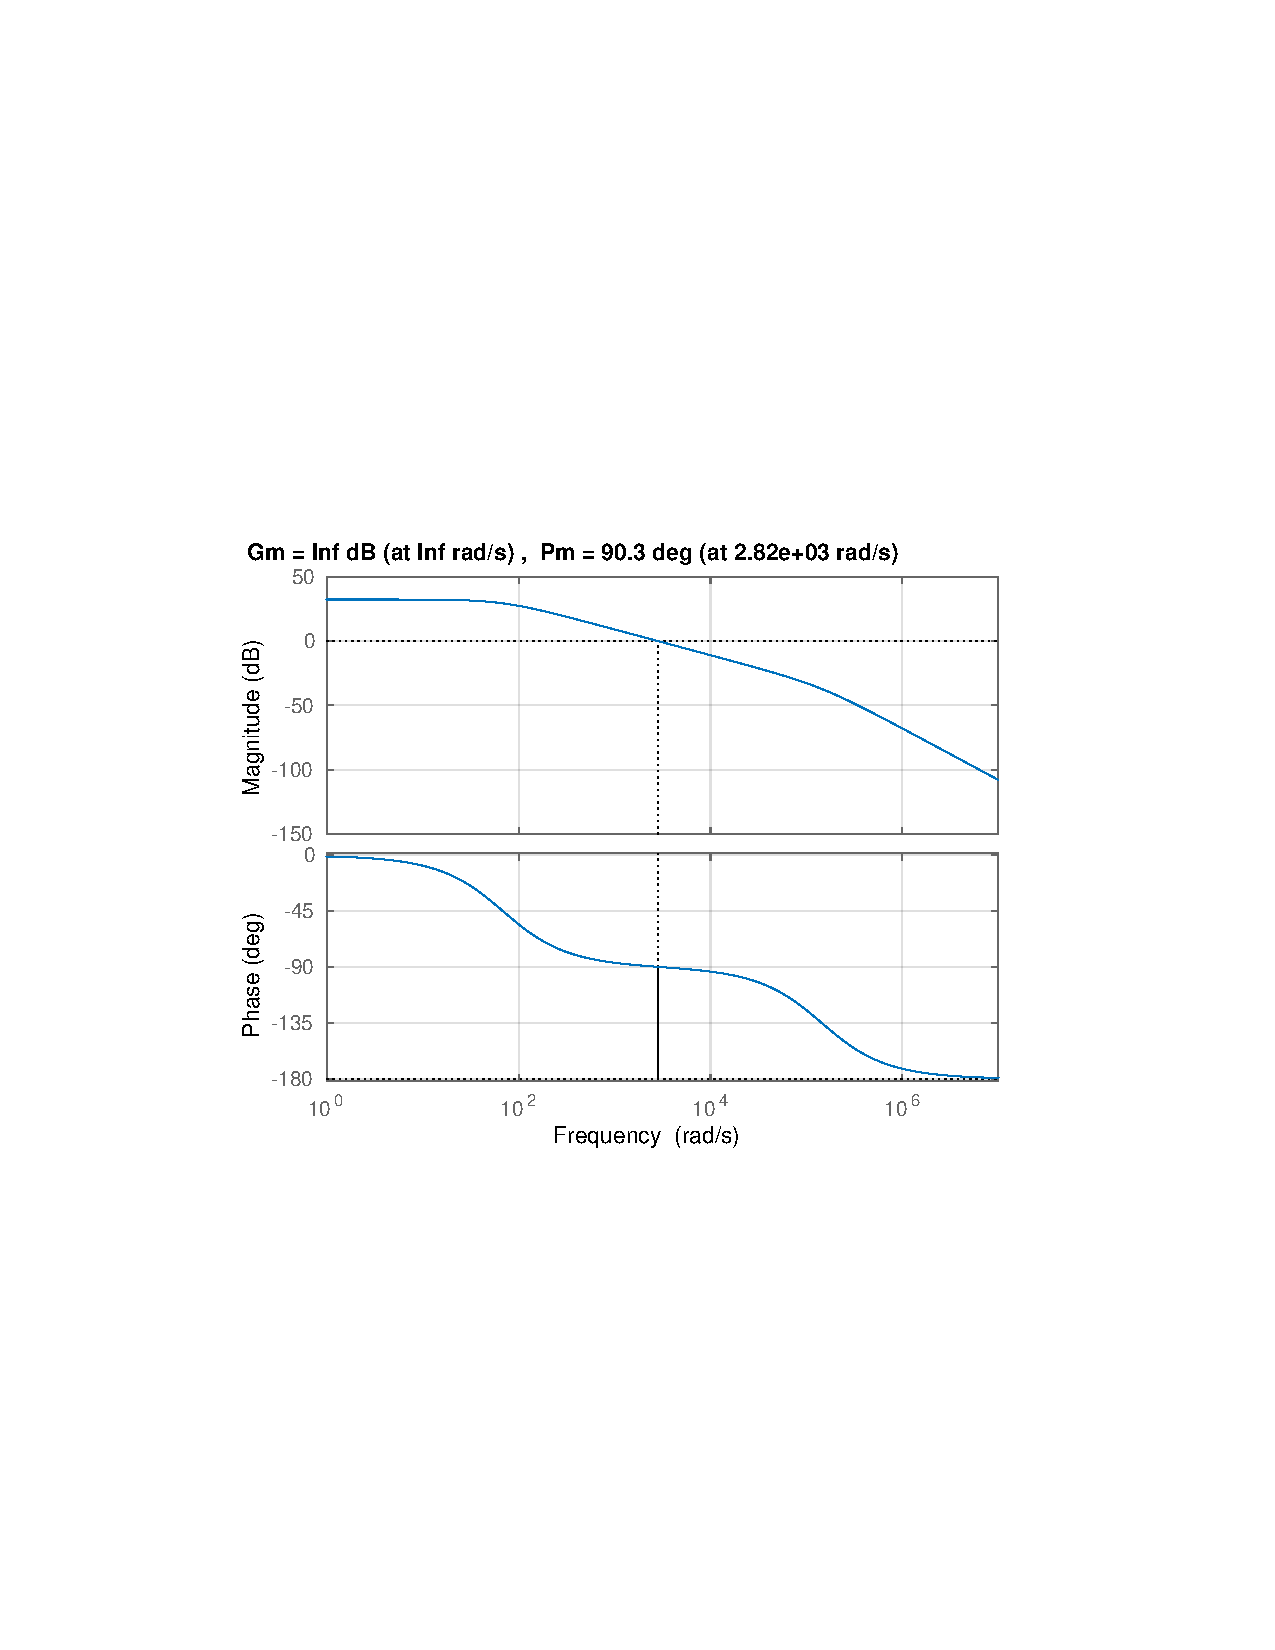
\includegraphics[width=.8\textwidth, trim=100 240 80 252, clip]{bode2}
	\caption{Szabályozási kör Bode-diagramja}
	\label{fig:bode2}
\end{figure}

%}}}

%{{{ Súlyfüggvény
\subsection{Súlyfüggvény}

A súlyfüggvényt könnyen kirajzolhatjuk az \verb|impulse| függvénnyel. Az alapjel
a névleges szögsebesség fele, vagyis
\begin{equation}
	\Omega_0 = \frac{\omega_\text{n}}{2} = 231.96~\frac{\text{rad}}{\text{s}}.
\end{equation}

\begin{figure}[H]
	\centering
	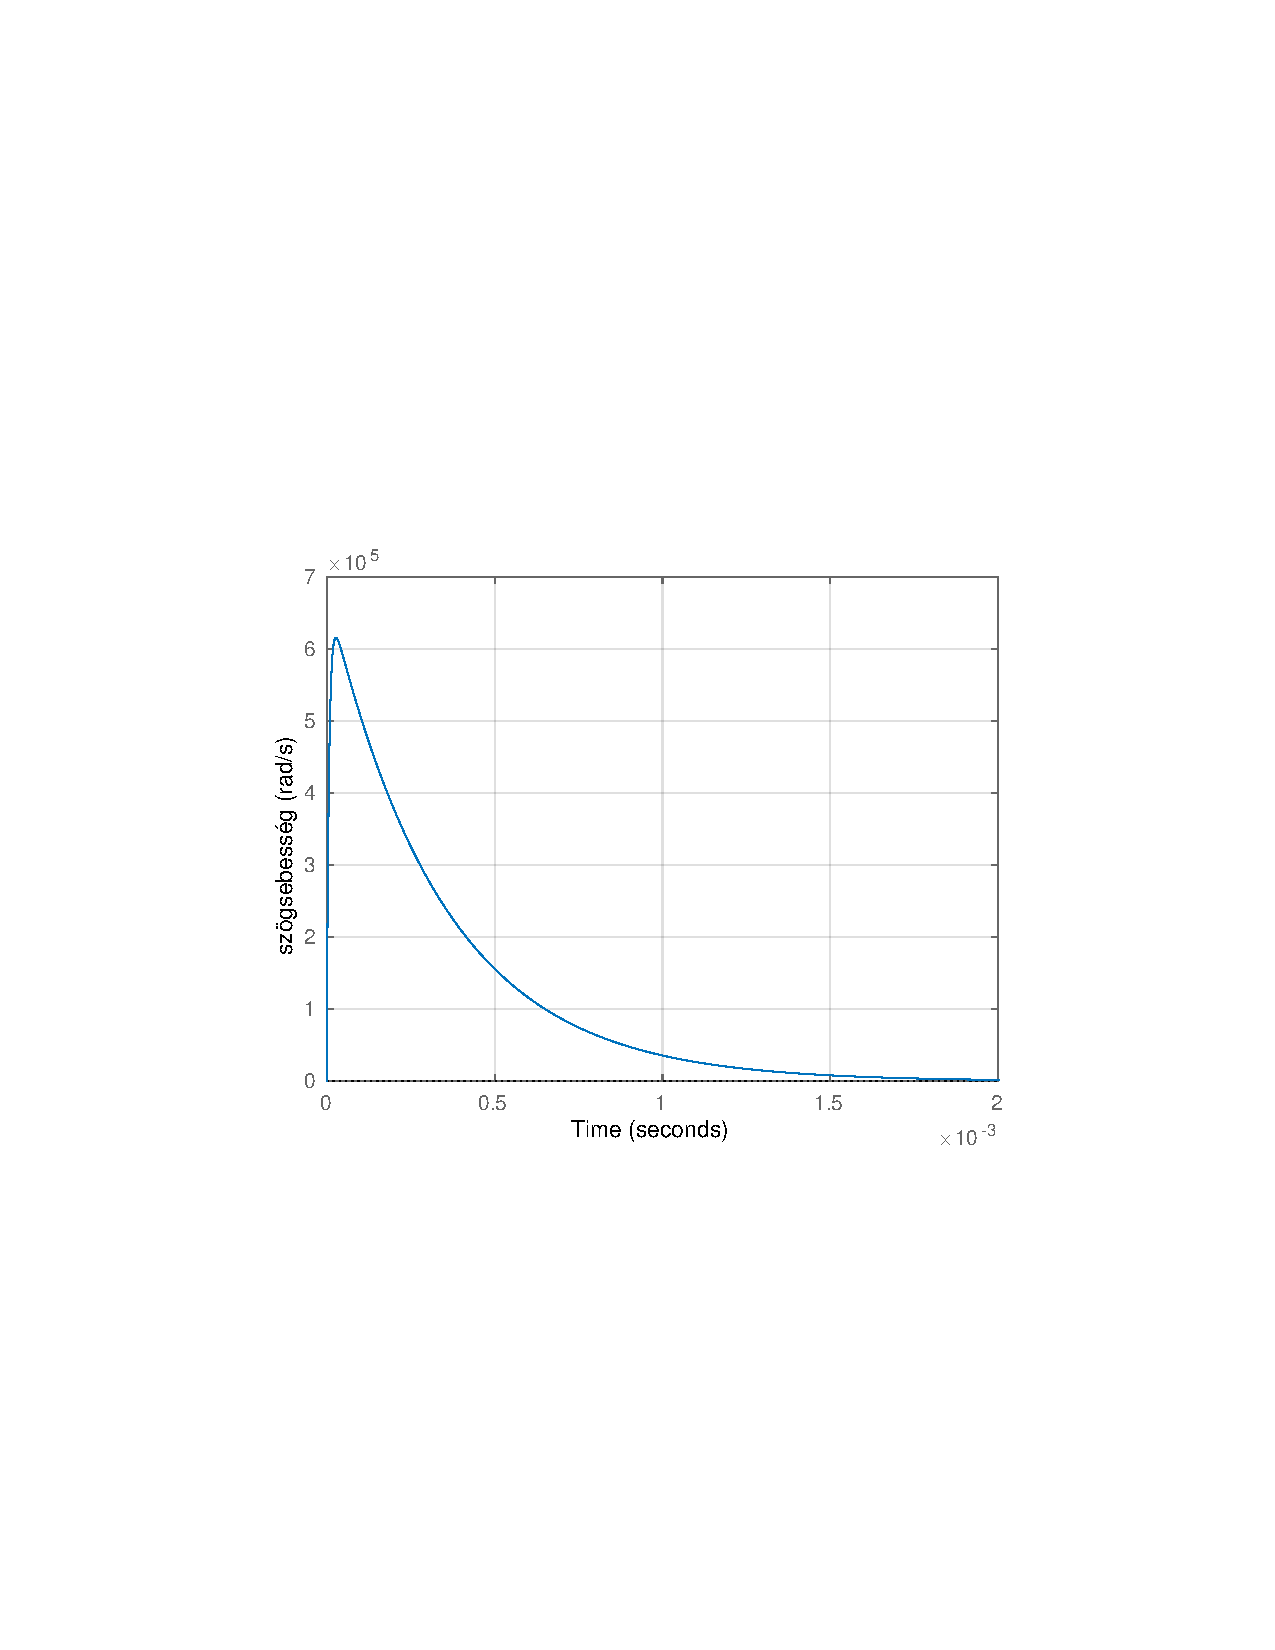
\includegraphics[width=.7\textwidth, trim=100 240 80 252, clip]{impulse2}
	\caption{A zárt szabályozási kör impulzusválasza}
	\label{fig:impulse2}
\end{figure}

%}}}

%{{{ Átmeneti függvény
\subsection{Átmeneti függvény}

Az átmeneti függvényt a \verb|step| függvény adja meg.
Az alapjel itt is a szögsebesség fele.

\begin{figure}[H]
	\centering
	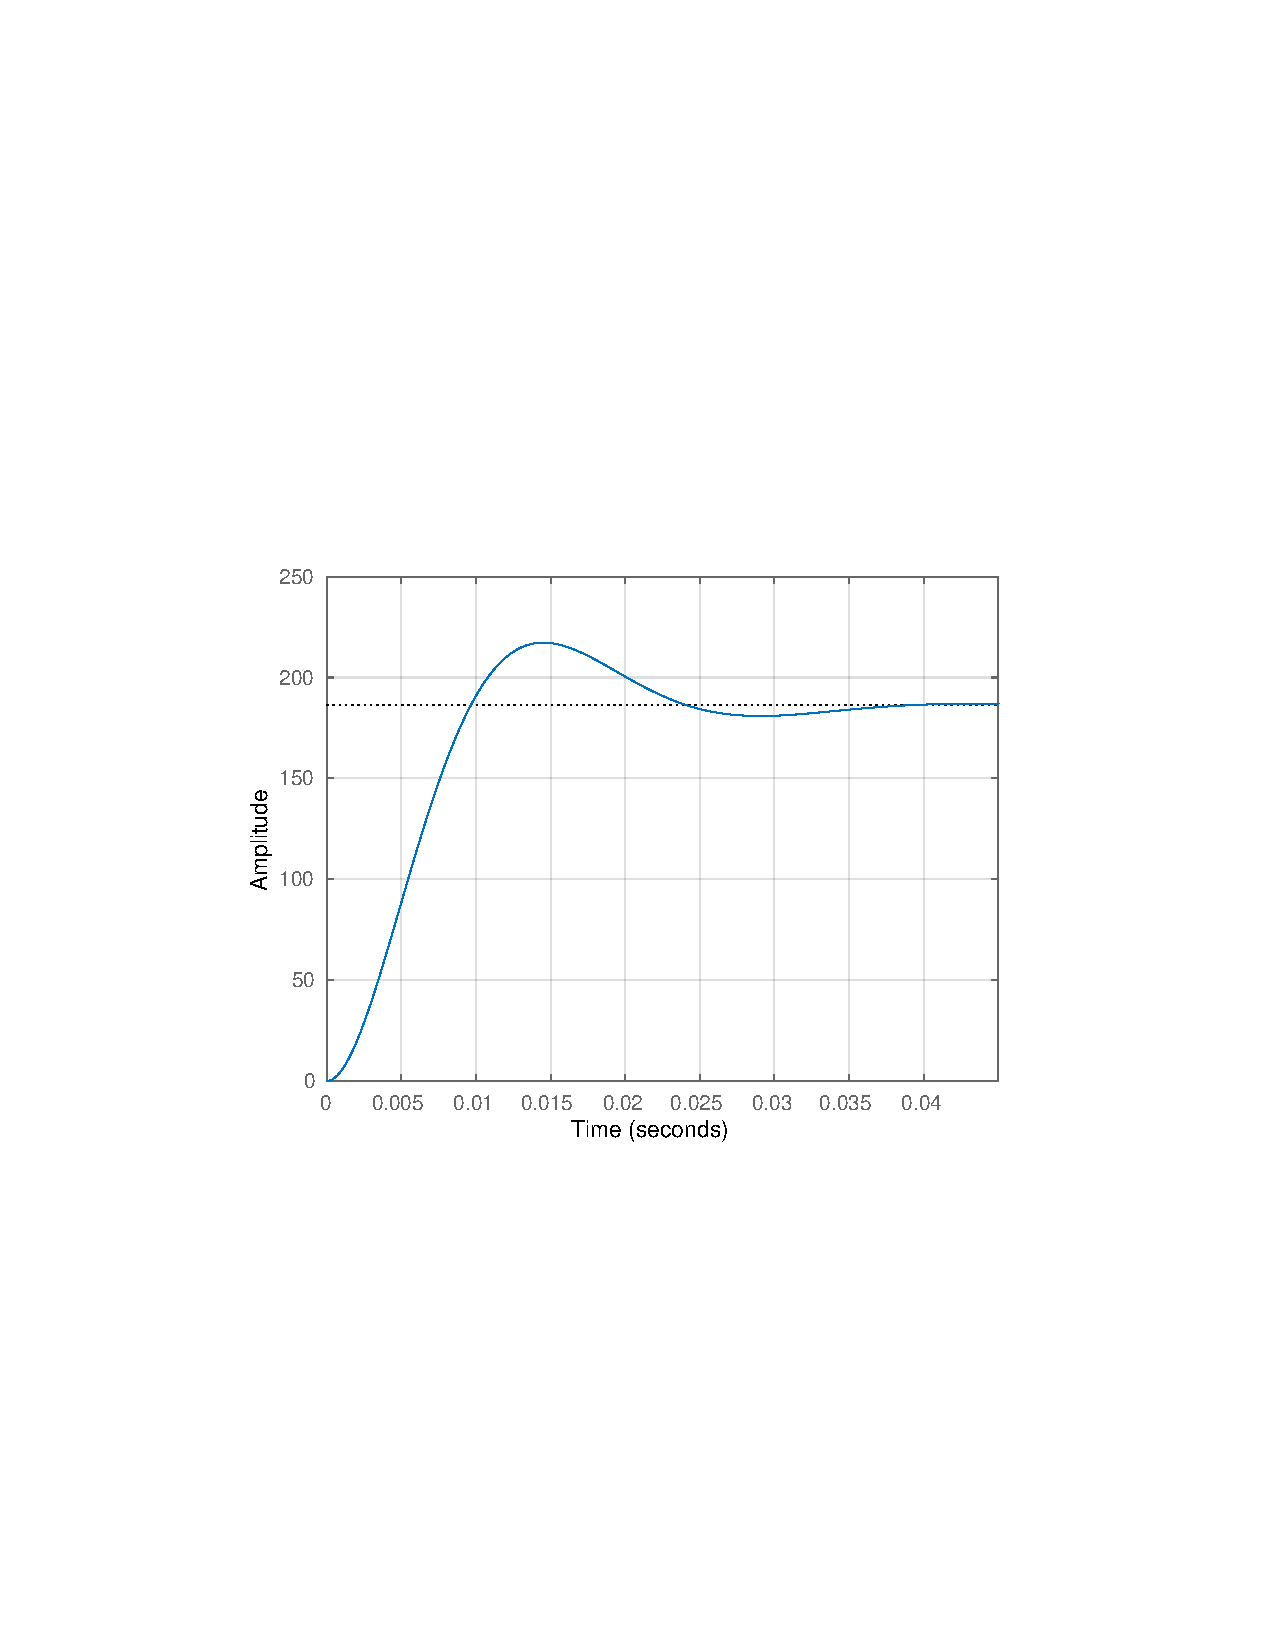
\includegraphics[width=.7\textwidth, trim=100 240 80 252, clip]{step2}
	\caption{A zárt szabályozási kör átmeneti függvénye}
	\label{fig:step2}
\end{figure}

%}}}
